\chapter{Perspectives}\label{chap:Persp}%\addcontentsline{toc}{chapter}{\nameref{chap:Persp}}
%\markboth{PERSPECTIVES}{}
\vfill
\hrule \vspace{.5cm}
{\hypersetup{linkcolor = black}
\localtableofcontents
}%
\vspace{.5cm} \hrule
\vfill
\clearpage

%Il reste encore beaucoup à faire

%\begin{itemize}
%	\item \'Electroacoustique
%	\begin{itemize}
%		\item Contrôle actif du champ acoustique
%		\item Changement de source principale
%	\end{itemize}
%	\item CFD
%	\begin{itemize}
%		\item Sunfluid
%	\end{itemize}
%	\item Expérimental
%	\begin{itemize}
%		\item Convection naturelle avec charge thermique au CHX
%	\end{itemize}
%\end{itemize}


\section{\'Electroacoustique}

Dans l'optique de poursuivre l'amélioration de cette pompe à chaleur thermoacoustique, l'aspect des sources acoustiques reste à considérer.

\subsection{Contrôle actif}
Le champ acoustique doit être contrôlé avec précision, en particulier l'impédance acoustique et son déphasage au sein du matériau poreux. Dans l'état actuel de la machine, les sources acoustiques sont contrôlées manuellement, et le déphasage inter-sources acoustiques est réglé sur le générateur de signaux. Une étude de l'asservissement de la source secondaire au moyen d'un dispositif de traitement du signal en temps réel tel que le \textit{digital signal processor} ADAU1701 de SigmaDSP (figure~\ref{fig:ActiveControl_ADAU1701}) ou un Teensy~4.1 (figure~\ref{fig:ActiveControl_Teensy41}) est proposée pour la suite de cette thèse, pour atteindre le champ acoustique optimal.



\begin{figure}[!ht]
    \centering
	\begin{subfigure}{.47\textwidth}
		\centering
		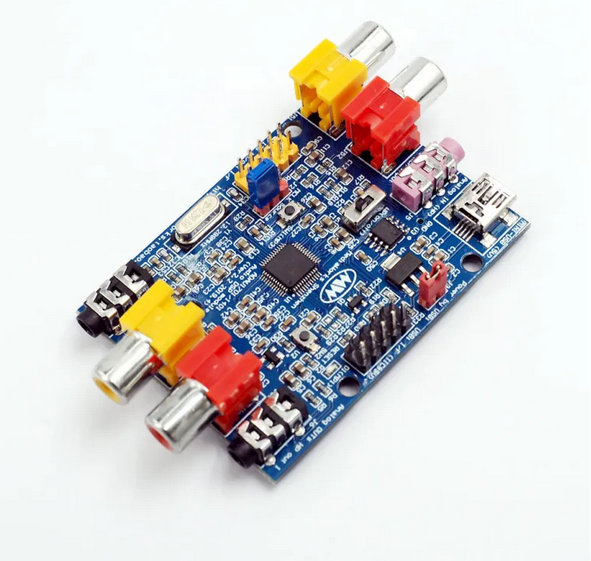
\includegraphics[height=6cm]{../fig/fig_ActiveControl/ADAU1701}
		\caption{}
		\label{fig:ActiveControl_ADAU1701}
	\end{subfigure}		
	\begin{subfigure}{.47\textwidth}
		\centering
		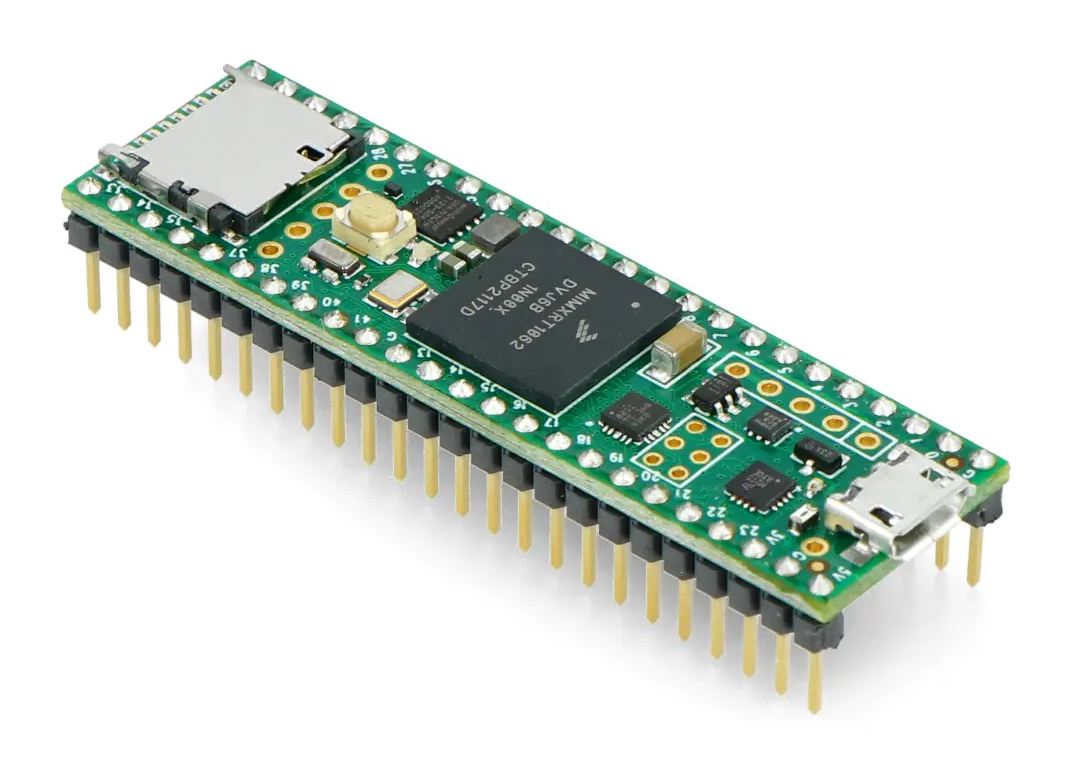
\includegraphics[height=6cm]{../fig/fig_ActiveControl/Teensy41}
		\caption{}
		\label{fig:ActiveControl_Teensy41}
	\end{subfigure}	    
    \caption{Dispositif de traitement du signal numérique en temps réel. \subref{fig:ActiveControl_ADAU1701} SigmaDSP ADAU1701 et \subref{fig:ActiveControl_Teensy41} Teensy 4.1}
    \label{fig:•}
\end{figure}

Ces cartes sont toutefois sources de retards : les différents calculs réalisés par le processeur, les filtres, les conversions analogique-numérique et numérique-analogique prennent du temps, mais il est possible d'atteindre des retards faibles de l'ordre de \qty{80}{\micro\second}, ce qui correspond à un déphasage de \ang{1.35} à la fréquence de fonctionnement du \textsc{Tacot}, \qty{47}{\hertz}.
\subsection{Remplacement des sources}

\section{Expérimentations supplémentaires}